\subsection{Government and Licensing}

In \CVCV, Government and Licensing are opposing forces:
While Government inhibits the melodic expression of
its target, Licensing makes it stronger.

Where in \cite{scheer2004} both forces are independent
from each other (a constituent can be both governed
and licensed, in which case both forces cancel out),
\cite{scheer2012} refines the model as follows:
\blockquote[\cite{scheer2012}]{
  (68) government over licensing
  
  no constituent can be governed and licensed at the
  same time. In case a constituent can potentially be
  subject to both lateral forces, it will be governed.
}

Each Nucleus always \wordunsure{exhibits}
all available forces: full vowels govern and license
while the ability of schwa and final empty Nuclei to
govern/license is subject to (separate) language-specific
parametrization.
In german, both schwa and final empty Nuclei govern but
do not license.

\TODO{concept: relations have a head}\par
\TODO{long vowels: complement needs to be licensed}

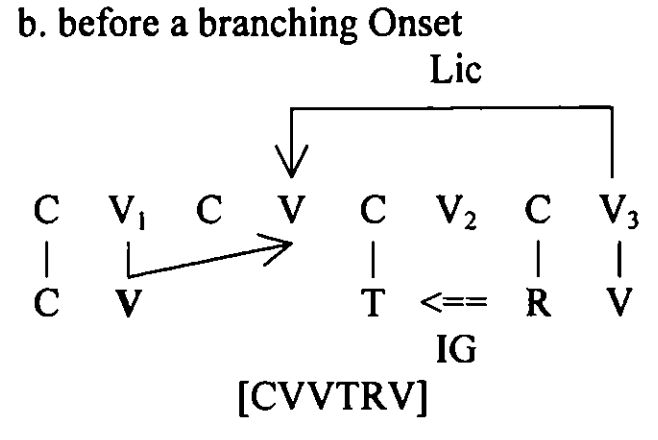
\includegraphics[width=.5\textwidth]{figures/lic-over-branching-onset.png}
